\chapter{Introduction}
  \section{Overview}
  Microseconds after the Big Bang, the Universe existed in a state known as
    the Quark Gluon Plasma (QGP).
  In the QGP, quarks and gluons are not in hadronic bondage, forced to 
    the confines of bound states such as protons and neutrons.
  The Large Hadron Collider (LHC) produces QGP in the lab in lead-lead (PbPb)
    collisions.
  The high energies and rates of the collisions at the LHC make it possible 
    to do detailed studies of the QGP. 
  The LHC is producing rare experimental probes such as suppressed jets and 
    heavy quarkonia at an unprecedented rate in heavy ion collisions. 
  As a result of recent LHC studies, physicists now have better constraints on 
    the properties like temperature, viscosity, and energy density of the QGP.

  The detailed studies of PbPb collisions coming out of the LHC 
    experiments require an understanding of the initial state of the ions 
    before they collide.
  Without more knowledge of the initial state, physicists cannot determine 
    which experimental effects are due to the QGP and which effects are 
    inherent to the nuclei themselves. 
  For example, suppression of heavy quarkonia is a signature of the QGP 
    but also appears to occur in deuterium-gold collisions where the QGP is not
    expected to arise \cite{dAuOniaPHENIX}. 
  Another important example is measurement of the viscosity, which depends on 
    the relationship between the observed azimuthal anisotropy and the 
    initial eccentricity of the overlap of the two colliding nuclei. 
  A clean probe of the initial state is needed by physicists to comprehensively 
    understand the QGP.
  Ultra-Peripheral Collisions (UPC) at the LHC provide such a probe.

  The current understanding of heavy ion collisions evolved over the
    last 30 years.
  Relativistic heavy ion collisions were first studied using the 
    Alternating Gradient Synchrotron (AGS) at Brookhaven National Lab (BNL) 
    in Upton, NY, followed by the Super Proton Synchrotron (SPS) at CERN near 
    Geneva, Switzerland. 
  From the numerous AGS and SPS experiments two main observables emerged,
    namely, \JPsi{} suppression and strangeness enhancement \cite{sps}. 
  These results pioneered the search for the QGP. 

  The AGS and SPS experiments were fixed target experiments.
  At AGS the ion isotopes $^{16}$O, $^{28}$Si, and $^{197}$Au beams were 
    collied with fix targets. 
  At SPS the same fix target configuration was used, but the ion isotopes were 
    $^{16}$O, $^{32}$S, and $^{208}$Pb.
  The center of mass energies per nucleon pair for these experiments ranged
    from just below 5 GeV to 20 GeV. 
  The threshold for creating the QGP requires an energy density of 0.15 
    $\sim$ GeV/fm$^{3}$ and a temperature near 170 MeV \cite{qgpThresh}.
  AGS and SPS just barely reached this threshold.
  Though the strangeness enhancement and \JPsi{} suppression 
    signals indicated that there was likely a deconfined state of quarks 
    and gluons created, at the energies of the AGS and SPS this state perished 
      to quickly to study any of its properties. 

  Plans for a colliding beam machine dedicated to heavy ions was first 
    proposed 1983.
  The proposed machine was designed to reach energies of 200 GeV per nucleon.
  At these energies, the QGP would presist long enough, and a that signs of
    a gas of hot quarks and gluons would emerge.
  In the summer of 2000 RHIC began collisions and the four experiments,
    STAR, PHENIX, BRAHMS, and PHOBOS started taking data. 
  With collision energies of 200 GeV per colliding nucleon, the energies 
    at RHIC were a factor of 10 higher than was previously achieved. 
  RHIC experiments confirmed for the first time the presence of a thermalized 
    state of quarks and gluons.
  Contrary to expectations, the state found at RHIC was found to be 
    strongly coupled fluid with nearly no viscosity \cite{}.

  The LHC heavy ion program began collisions in 2010, colliding PbPb at 
    a center of mass energy of 2.76 TeV per nucleon pair. 
  This corresponds to an increase in the colliding energy by an order of 
    magnitude with respect to RHIC. 
  The LHC experiments, ALICE, ATLAS, and CMS have studying the heavy ion 
    collisions since then. 
  In 2013 LHCb joined the LHC heavy ion program. 
  Thanks to the LHC and RHIC physics programs, a new era of precision
    heavy ion measurements is underway. 

  The latest results from the LHC have come from the 2013 proton-lead (pPb)
    run.
  This period of data taking was originally designed to be a control 
    measurement.
  For example, the initial suppression signals observed in dAu collisions at 
    RHIC were believed to be due to non-QGP effects \cite{ }. 
  The azimuthal anisotropy of particles present in PbPb and AuAu at the LHC and 
    RHIC respectively were believed to be signals of flow from the QGP and 
    would not appear in the lower density pp and pPb collisions.
  However, CMS showed evidence of a flow signal in high multiplicity pp events
    in early 2011 \cite{ }. 
  More recently ALICE has shown a structure in two particle correlation 
    measurements, referred to as the double ridge \cite{ }, and CMS and ALICE have both 
    shown an elliptical flow signal present in the pPb data \cite{}.

  The latest data from the pPb and dAu measurements confirm the need to 
    understand the nature of the initial state. 
  UPC events fulfill this need by probing the nucleus through photon 
    interactions.
  By measuring UPC \JPsi{} events, theoretical models of the initial state can 
    be constrained.
  In this thesis, the CMS capability for measuring this process, the 
  description of the analysis, and the comparison between the measured 
    coherent \JPsi{} cross section to theoretical models are given. 

  \section{Confirmation and characterization of the QGP from HI measurements}
    Creation of the QPG can be confirmed by comparing the measured energy 
      densities with predicted critical temperature and energy densities
      from lattice QCD measurements. 
    The critical energy density, $\epsilon_{crit}$, and critical temperature, 
      $T_{crit}$, are calculated to be 1.5 GeV and 170 MeV from lattice QCD 
      estimates \cite{ }.
    The measurement of the $\frac{dE_{T}}{d\eta}$ provides a means of 
      estimating the energy density of the hot state created in heavy ion
      collisions. 
    The temperature can be estimated from the transverse momentum, \pt{}, 
      spectrum of the direct photons, photons that come directly from the 
      QGP.
    At both RHIC and the LHC the energy density and temperature were found to 
      be well above the critical values. 
    The measurements from CMS and ALICE at the LHC and STAR and PHENIX at RHIC
      confirm that the critical values for energy density and temperature are
      exceeded.

    The value of $\frac{dE}{d\eta}$ measured by CMS \cite{cmsEt} and PHENIX 
      \cite{phenixDeDeta} was done using the expirements' calorimeter systems.
    The value of $E_{T}$ for this measurement is defined as 
      $E_{T}=\sum_{i}E_{i}sin\theta_{i}$, where $E_{i}$ is the energy measured 
      by the ith calorimeter element and $\theta$ is the angle between the 
      center of the detector element and the interaction point. 
    The calculated $\frac{dE_{T}}{d\eta}\bracevert_{0}$, the interval 
      $0.35<|\eta|$ was used by both experiments and corrisponds to the full
      coverage of the PHENIX calorimeters. 
    From the $\frac{dE_{T}}{d\eta}\bracevert_{0}$ measurements, the energy 
      density of the created medium at the LHC and RHIC were estimated from the
      Bjorken energy density formula, 
      $\epsilon_{Bj}=\frac{1}{A\tau}\frac{dE_{T}}{dy}$, where $A$ is the region
      of overlap between the two colliding nuclie and $\tau$ is the formation
      time of the medium \cite{bjEdense}.
    The energy density, $\epsilon{Bj}\dot\tau$, from PHENIX was measured at
      RHIC to be 5.4$\pm$0.6 GeV fm$^{-2}$c$^{-1}$ for the 5\% most energetic 
      collisions compared to the 14 GeV fm$^{-2}$c$^{-1}$ at the LHC as 
      measured by CMS. 
    Both values are well above $\sim$ 1.5 GeV fm$^{3}$ critical energy density
      calculated from lattice QCD when assuming a medium formation time $\tau$ 
      = 1fm/c.
      \begin{figure}[!Hhbt]
        \centering
        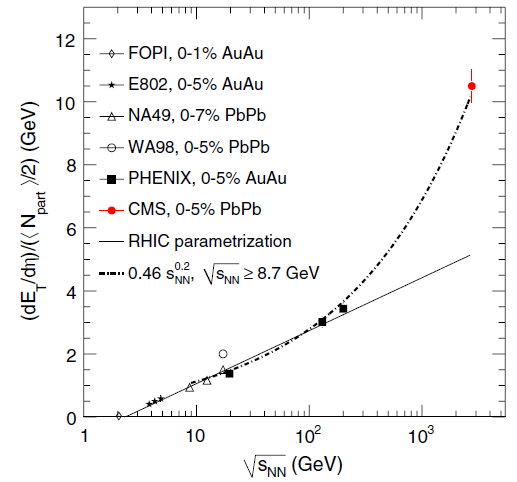
\includegraphics[width=.65\textwidth]{dEtdEta}
        \caption{Comparison of $\frac{dE_{T}}{d\eta}$ as a function of 
          collision energy, $\sqrt{s_{NN}}$, normalized by the number 
          participating nucleons, $N_{p}$, to account for the difference in 
          the ion species collided at the various different experiments.}
        \label{fig:dEtdEta}
      \end{figure}

    Direct photons, thermal photon created in the QGP, have been measured 
      at RHIC by PHENIX \cite{phenixPhoton2010} and at the LHC by ALICE 
      \cite{photonALICE} through the measurements of electron-positron pairs.
    Each experiment measured the inclusive \pt{} spectrum from 
      electron-positron pairs, all pairs from the sample are taken without
      regard to the creation mechanism.
    The PHENIX measurement was taken from pp collisions and top 20\% most 
      energetic AuAu collisions, collisions with a centrality of 0-20\%. 
    The ALICE measurement analyzed the 0-40\% centrality, 40\%-80\% centrality
      PbPb collisions, and pp collisions. 
    In both measurements, the contribution to the inclusive spectrum was sorted 
      into a direct component and a component from background, primary decays
      from hadrons such as pions and eta. 
    In the PHENIX measurement this was done by preforming a fit to the mass 
      distribution of the electron-positron pair for each \pt{}.
    For the ALICE measurement, the double ratio between the inclusive photons 
      to pions over the ratio between photons from hadron decays and pions was
      measured to estimate the direct contribution. 
    The inclusive photon \pt{} were then rescaled by the direct photon 
      fractions to produce a direct photon spectrum.
    The slope of an exponential fit to the low \pt{} portion the direct photon 
      spectrum is used to measure the temperature.
    \begin{figure}[!Hhbt]
      \centering
      $ \begin{array}{c c}
        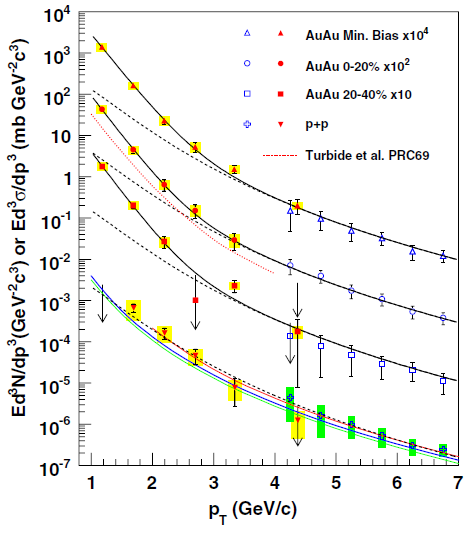
\includegraphics[width=.4\textwidth]{phenixDirectPhoton} &
        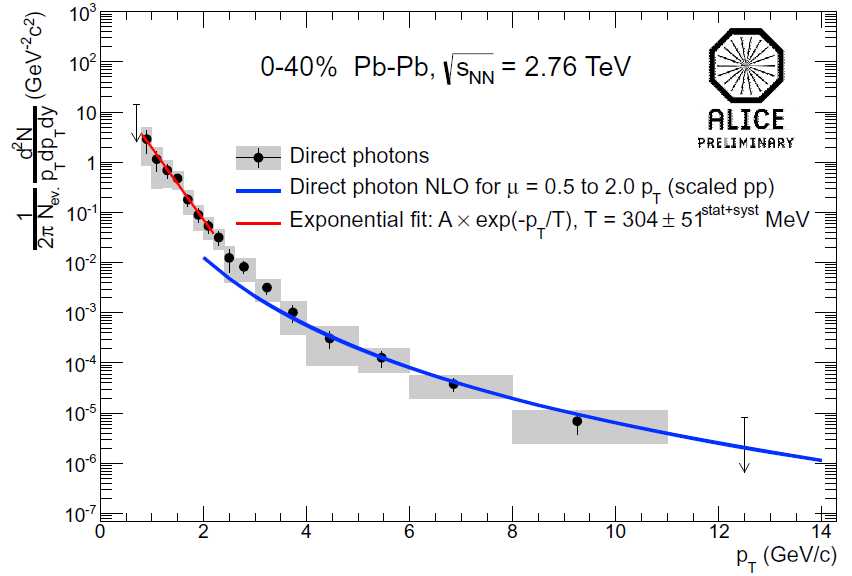
\includegraphics[width=.55\textwidth]{aliceDirectPhoton}
      \end{array} $
      \caption{Direct photon invariant yield as a function of \pt{} from 
        PHENIX \cite{phenixPhoton2010} (left) and ALICE \cite{photonALICE} 
        (right)}
      \label{fig:directPhotonPt}
    \end{figure}

    The direct photon through measurement of the temperature offers a clear 
      way of establishing whether the critical temperature for deconfinement
      was achieved. 
    The direct photon \pt{} spectra in Fig.~\ref{fig:directPhotonPt} show a 
      clear enhancement at low \pt{} compared to the rescaling to the pp 
      spectra that fits the high \pt{} part of the spectrum, indicating a 
      clear deviation for pp collisions.
    The low \pt{} photons therefore primarily come directly from the thermal 
      activity of the QGP.
    The thermal spectrum of the QGP is therefor imprinted on this part of the 
      spectrum.
    The exponential fits to the spectra provide this temperature. 
    The temperature from PHENIX was measured to be 221 $\pm$ 21 MeV and 
      304 $\pm$ 51 MeV from ALICE, both well above the critical temperture
      estimated from lattice QCD of $\sim$ 170 MeV.

    The combination of the energy density and temperture measurements are RHIC
      create a consistent picture, both RHIC and the LHC have created a 
      deconfined state, and due the higher collision energies at the LHC the 
      the medium gets hotter. 
    
    Prior to the RHIC, the QGP was thought to be a gas of quarks and gluons.
    At RHIC the measurements at STAR showed that the medium appeared to obey 
      hydrodynamic equations and flows like a fluid.
    This same signal was also measured by CMS at the LHC. 

    This is how you measure elliptic flow is measured.

    These are the results. 

    The signal indicates that there is very little viscosity. 
    However, this depends on the eccentricity of initial overlap region, which
      depends on the description of the initial state of the colliding nuclei.

    \begin{figure}[!Hhbt]
      \centering
      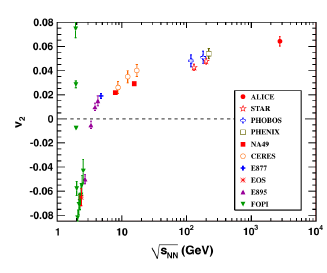
\includegraphics{elipFlow}
      \caption{ $v^{2}$ elliptical flow measurements from SPC to the LHC.}
      \label{fig:elipFlow}
    \end{figure}

     \begin{figure}[!Hhbt]
      \centering
      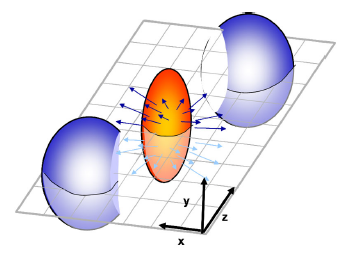
\includegraphics{elipFlowSchem}
      \caption{ Elliptical flow schematic diagram.}
      \label{fig:elipFlowSchem}
    \end{figure}

  \section{Recent results from HI control measurements}

    \subsection{The HI collision}
      The AGS and SPS created the first signs of a deconfined state, but the 
        nature of the state was uncertain.
      At RHIC the existence of the QGP was confirmed and it's nature found to 
        be hydrodynamic.
      The LHC and RHIC experiments are now looking deeper in the characteristics
        of QGP.
      More precise and sophisticated measurement techniques now require a 
        better understanding of the ions before they collide in order to 
        produce the proper theoretical modeling. 

      Over the course of the experimental evolution the following picture of 
        a heavy ion collision emerged. 
      First, highly contracted ions travel toward each other.
      Second, QGP forms and reaches thermal equilibrium.
      Third, this hot dense state expands hydrodynamically.
      Fifth, Fifth as the collection of quarks and gluons cool, a gas of hot
        hadrons forms and expands.
      Finally, all interactions freeze out and the produced particles stream 
        to the detector. 
